\documentclass{article}
\usepackage[utf8]{inputenc}
\usepackage{graphicx}
\usepackage{geometry}
\usepackage{hyperref}

\newgeometry{
    top=0.75in,
    bottom=0.75in,
    outer=1in,
    inner=1in,
}

\title{Projet APO {\Large Tic-tac-toe 3D}}
\author{Boissot Aurélien, Laqueuvre Damien, Moulon Florent}
\date{janvier 2023}

\begin{document}

\maketitle

\renewcommand{\contentsname}{Table des matières}
\tableofcontents
\newpage

\section{Structure de l'archive}
\begin{itemize}
    \item Les classes .java sont dans le dossier \textit{ /projet\_tictactoe/src/main/java/apo/boissot\_laqueuvre\_moulon}
    \item La documentation est dans le dossier \textit{ /Javadoc}
    \item Les diagrammes UML sont dans le dossier \textit{ /Rapport/Diagramme UML}
\end{itemize}



\section{Méthodologie}
Après avoir pris connaissance du sujet, nous avons décidé de mettre en commun nos idées avant de commencer à programmer.

\subsection{Choix des outils}
 La première étape a été de décider quels outils nous allions utiliser pour la réalisation du projet.\\ \\
 
 Nous avons rapidement choisi d'utiliser les outils qui nous étaient familiers, à savoir :
 \begin{itemize}
    \item Visual Studio Code \textit{comme IDE}
    \item Java 8 \textit{comme version de java car c'est la version que nous connaissons le mieux et que nous n'avons pas besoin des nouveautés introduits par les versions postérieures}
    \item GitHub \textit{pour le travail collaboratif et le versioning}
    \item StarUML \textit{pour créer les diagrammes UML}
\end{itemize}
De plus, il nous a semblé intéressant d'essayer un outil de gestion de chaîne de compilation. Notre choix s'est porté sur Maven.\\


 \subsection{Choix de l'architecture}
 Après s'être mis d'accord sur notre espace de travail, nous avons échangé autour des grandes lignes de notre application.\\ \\
 
 Pour cela, nous avons réalisé un premier diagramme de classe sommaire. C'est à ce moment que nous avons décidé qui les Grille2D et Grille3D seraient remprésentées par 2 classse héritant d'une même classe abstraite Grille.\\
 Nous avons décidé de séparer le lancement du jeu et la partie en elle-même dans 2 classes différentes.\\
 Enfin, nous avons choisi de représenter les joueurs (humain ou IA) par une classe.\\

 Nous avons également choisi dès le départ les extensions que nous souhaitions implémenter afin d'adapter la conception en conséquence, notamment pour les grilles de taille variable. \\

 
 \subsection{Déroulement temporel}
Une fois que les bases du projet furent établies, nous nous sommes lancés dans la programmation.\\ \\

La première étape fut de créer le squelette de la classe Grille et Grille2D, afin d'inplémenter toutes les fonctions élémentaires des grilles. Un test régression a également été créé dans la foulée pour tester les fonctions et s'assurer qu'elle resteront correctes tout au long du projet.\\
Pour éviter d'avoir à repenser toutes ces fonctions plus tard, nous avons décidé de directement considérer nos grilles comme étant de taille variable.\\ \\

Une fois ce squelette en place, nous avons créé les classes relatives au coeur du jeu et en parallèle nous avons adapté les fonctions de Grille2D dans Grille3D.\\
Le principal défi fut la gestion des inputs utilisateur. Entre la vérification des données et la gestion des Scanners java, cette étape fut plus longue que prévu.\\
Nous avons aussi retravaillé l'affichage pour qu'il soit plus agréable avec les grilles de grande taille.\\
A la fin de ces étapes, nous avions un jeu fonctionnel où 2 joueurs humains poouvais s'affronter sur une grille de taille n en 2 dimensions. La version en 3 dimensions fut terminée quelques temps après.\\ \\

Dès que le jeu de base commençait à fonctionner, nous avons commencé à travailler sur les extensions optionelles que nous avions prévues.\\
Nous avons commencé par implémenter les plus simples en parrallèle, c'est à dire l'affichage de la combinaison gagnante et la sauvagarde.\\
Après quoi, nous avons codé le minmax et adapté le déroulement du jeu au mode humain/ordinateur.\\ \\

Pendant que certains finalissaient les détails, d'autres commençaient le rapport et remettaient au propre les diagrammes UML.\\


 
 \subsection{Répartition du travail}
Nous avons répartit au mieu les différentes taches en fonction de nos capacités et de nos envies tout au long du projet.\\
Pour cela, nous avons commencé par lister et se repartir les besoins immédiats. Puis, quand l'un de nous terminait sa tache, nous faisions un bilan pour supprimmer les taches effectuées, ajouter les nouveaux besoins et choisir sa prochaine action.\\
Voici un bilan des réalisations de chacun :\\ \\

\subsubsection{Aurélien}
 \begin{itemize}
    \item affichage Grille3D
    \item documentation de ses fonctions
    \item sauvegarde de la partie
    \item vérification des input pour la Grille3D
    \item gestion des Scanner et des inputs utilisateurs
    \item classe InterfaceJeu
\end{itemize}

\subsubsection{Damien}
 \begin{itemize}
    \item diagramme de cas d'utilisation
    \item vérification des victoires Grille2D
    \item vérification des victoires Grille3D
    \item documentation de ses fonctions
    \item mise en place de MinMax
\end{itemize}

\subsubsection{Florent}
 \begin{itemize}
    \item diagramme de classe
    \item méthodes basiques de Grille2D
    \item méthodes basiques de Grille3D
    \item affichage Grille2D
    \item Vérification des inputs pour la Grille2D
    \item rapport
    \item documentation de ses fonctions
\end{itemize}


\section{Extensions optionnelles}

\subsection{Extensions fonctionnelles}
\subsubsection{Taille variée \hfill 1 point}
Comme expliqué plus tôt, dès la conception nous avons pensé les Grilles comme des tableaux de taille n variable. Il a donc été très simple de prendre un paramètre n pour que le nombre de cases d’une Grille2D soit $n^{2}$ et celle d’une Grille3D, $n^{3}$.\\

\subsubsection{Affichage de la combinaison gagnante \hfill 1 point}
Lorsqu’un joueur gagne, nous affichons la grille une dernière fois. Les cases de la combinaison gagnante sont encadrés par des chevrons :
\begin{verbatim}
|>O< X  3 |
|>O< X  6 |
|>O< O  X |
\end{verbatim}

\subsubsection{Sauvegarde du jeu \hfill 1 point}
Lorsque l'on demande au joueur de saisir une case, il peut saisir "save" à la place de son choix de case et cela sauvegardera sa partie dans un fichier.\\ 
Lors de sa prochaine partie, un message s'affichera lui demandant s'il souhaite charger sa partie enregistrée. S'il accepte, sa partie précédente sera rechargée et il pourra continuer à jouer sur celle-ci.\\

\textbf{Structure de la sauvegarde :}
 \begin{itemize}
    \item La première ligne contient toutes les informations caractérisant la partie : le type de grille (2D ou 3D), le types de joueurs (joueur humain ou IA), qui commence la partie, et la taille de la grille.
    \item Les lignes suivantes contiennent les coup joués par les joueurs avant d'avoir sauvegardé : chaque ligne précise le symbole du joueur ("X" ou "O") et le coup joué.
\end{itemize}


\subsubsection{Intelligence artificielle 2D et 3D\hfill 2 points}
En plus du mode humain contre humain, notre programme propose un mode humain contre ordinateur.\\
Afin de faire une IA capable de jouer, nous avons implémenté l'algorithme minimax pour des parties en 2D et en 3D.\\

\subsection{Extensions techniques}
\subsubsection{Compilation automatisée \hfill 1 point}
Nous avons utilisé Maven pour automatiser la compilation et le lancement de notre programme.\\
Dans une console, placez vous dans le dossier \textit{ /projet\_tictactoe/}\\
 \begin{itemize}
    \item Pour compiler le code utiliser les commandes : \\
    \textbf{mvn compile \\
            mvn package \\
            mvn install}

    \item Pour lancer le programme, utiliser la commande : \\
    \textbf{java -cp projet\_tictactoe-1.0-SNAPSHOT.jar apo.boissot\_laqueuvre\_moulon.App}
 \end{itemize}


\subsubsection{Versioning du code \hfill 1 point}
Comme mentionné au début, nous avons utilisé GitHub pour le versioning de notre code.\\
le répertoire git utilisé est public et accessible ici : \\ \href{https://github.com/FlorentMoulon/Projet-APO-Tic-tac-toe-3D}{https://github.com/FlorentMoulon/Projet-APO-Tic-tac-toe-3D}\\

\subsubsection{Tests unitaires \hfill 1 point}
Des tests unitaires vérifiant la bonne exécution des méthodes principales de nos classes on été inmplémentés sous la forme de fonction testRegression().\\
Chaque classe possède une telle fonction qui effectue et affiche des test de toutes les méthodes. Ces fonctions sont tenues à jour tout au long du développement de l'application pour s'assurer que les nouvelles fonctions ne "cassent" pas les anciennes.\\

\newpage

\section{Diagrammes UML}

\subsection{Diagramme de cas d'utilisation}
\begin{figure}[h]
    \centering
    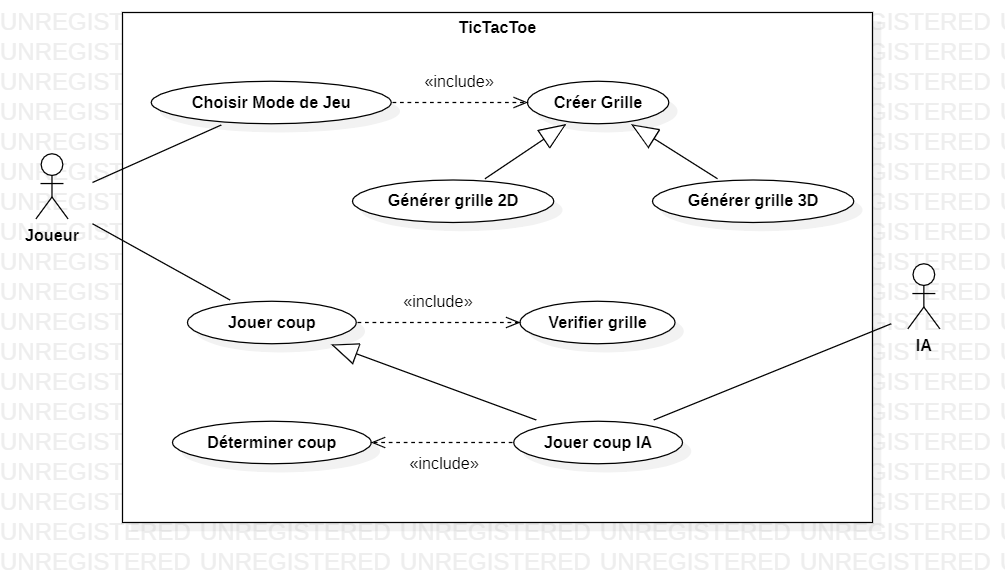
\includegraphics[scale=0.5]{Diagramme UML/Diagramme cas d'utilisation.png}
    \caption{Diagramme de cas d'utilisation}
    \label{fig:Diagramme de cas d'utilisation}
\end{figure}

\newpage
\subsection{Diagramme de classe}
\begin{figure}[h]
    \centering
    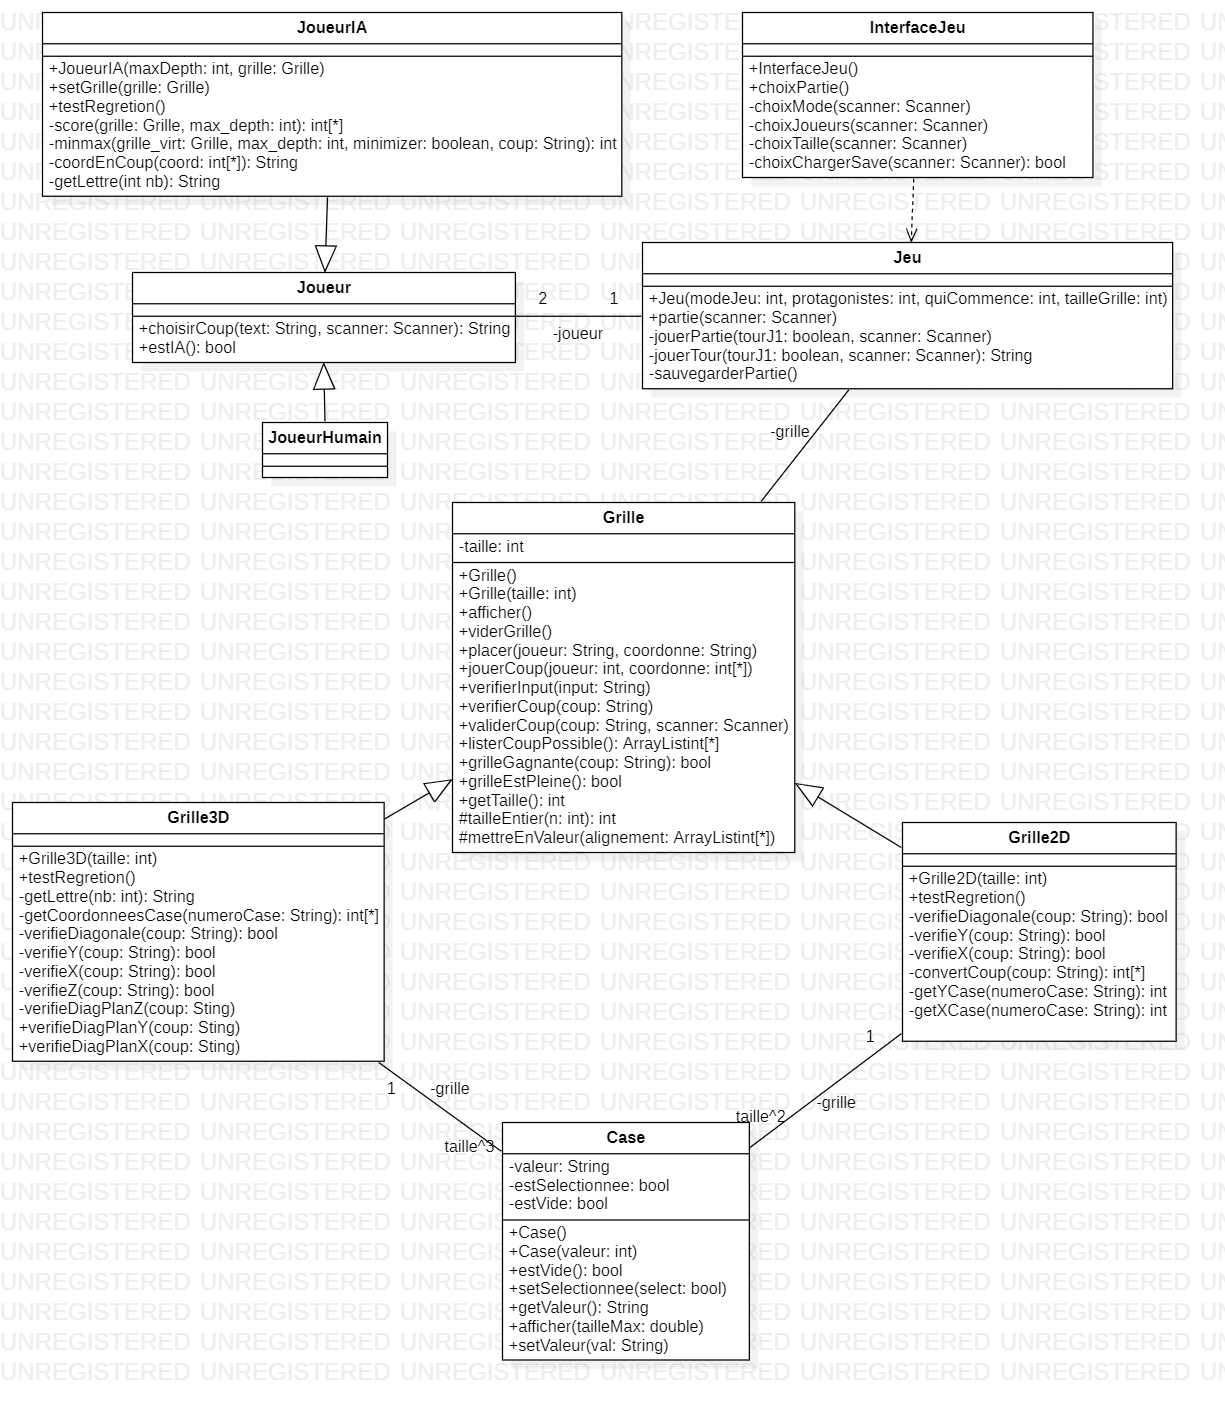
\includegraphics[scale=0.35]{Diagramme UML/Diagramme de classe.png}
    \caption{Diagramme de classe}
    \label{fig:Diagramme de classe}
\end{figure}

\newpage
\subsection{Diagramme de séquence}
\begin{figure}[h]
    \centering
    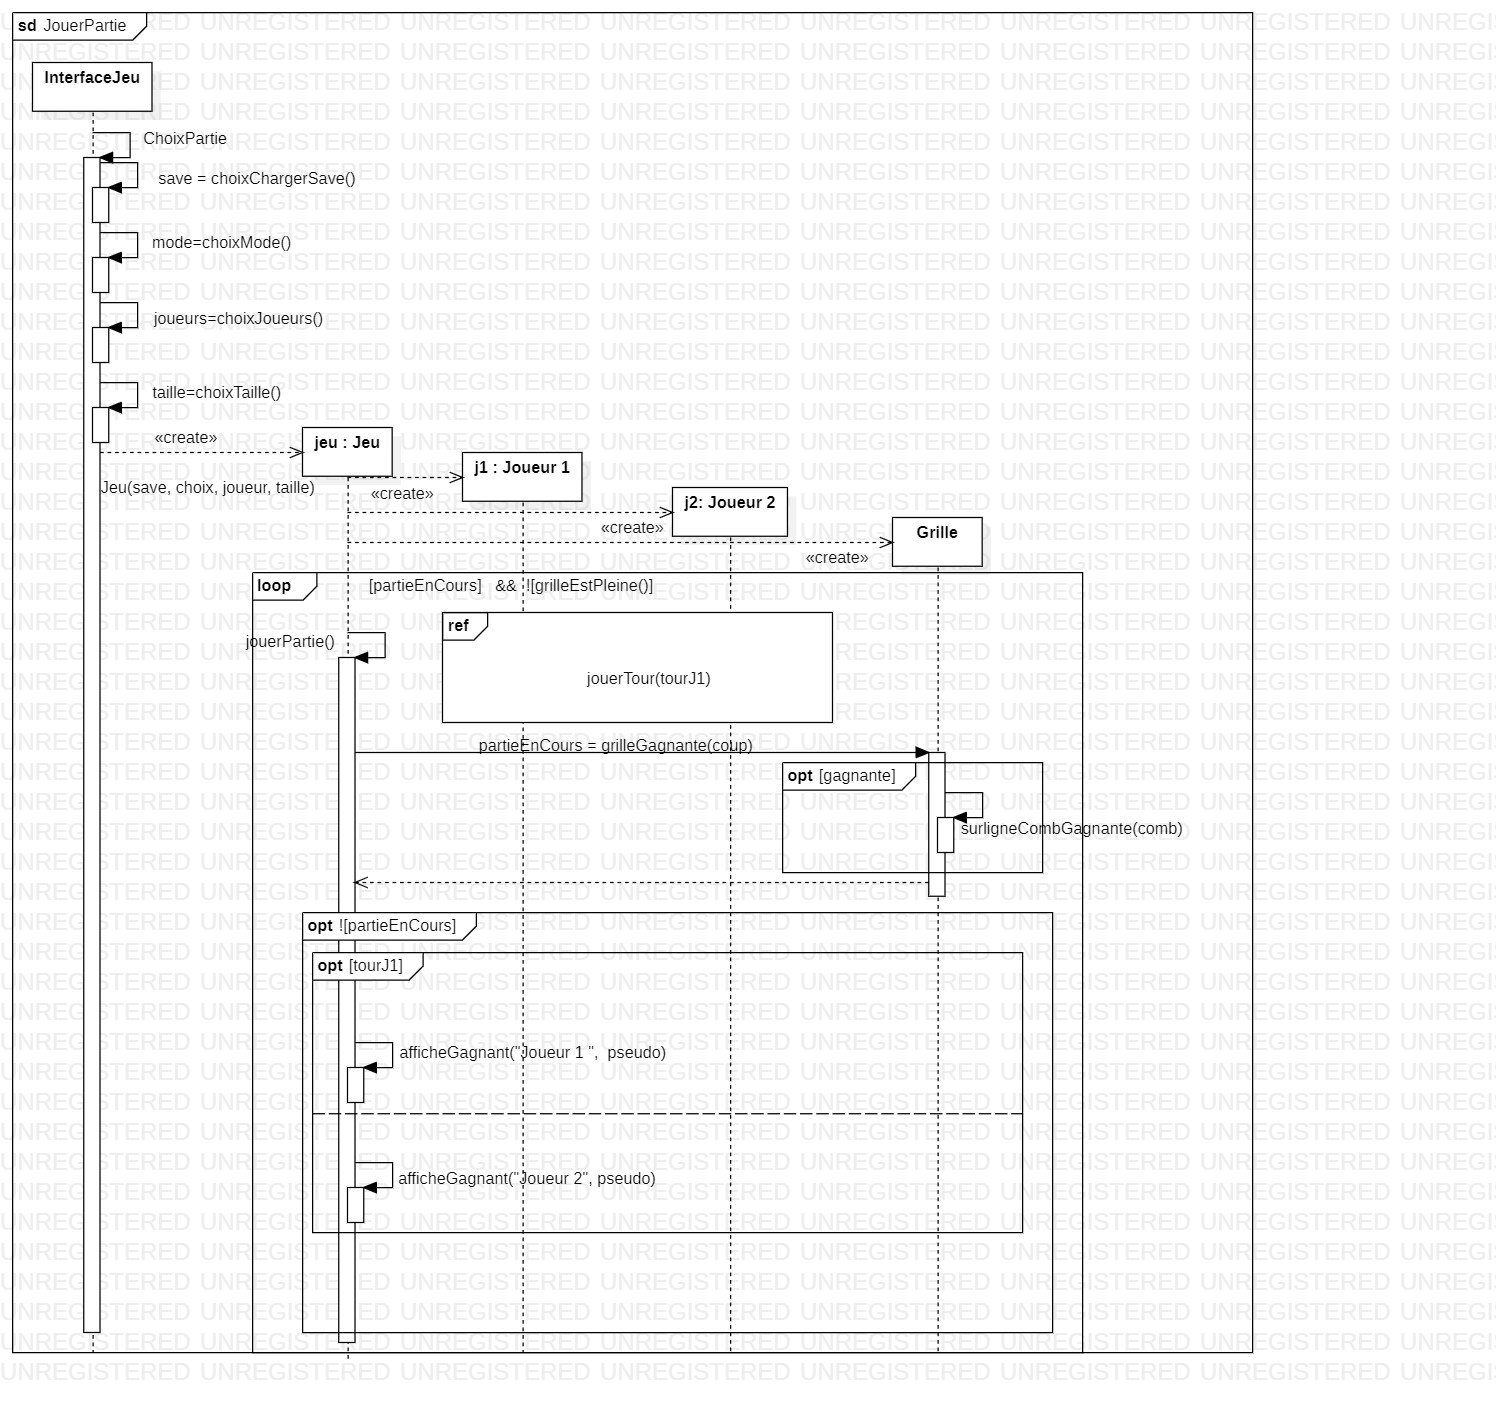
\includegraphics[scale=0.36]{Diagramme UML/Diagramme de sequence.png}
    \caption{Diagramme de séquence}
    \label{fig:Diagramme de séquence}
\end{figure}

\end{document}